%-*- coding: UTF-8 -*-
% Gougu.tex
% 勾股定理

\documentclass[UTF8]{ctexart}
\usepackage{graphicx}
%\usepackage[backend=biber]{biblatex}

\title{杂谈勾股定理}
\author{张三}
\date{\today}

\newtheorem{thm}{定理}          % thm environment

\begin{document}
    \maketitle

    \begin{abstract}
        这是一篇关于勾股定理的小短文。
    \end{abstract}

    \tableofcontents
    
    \section{勾股定理在古代}
        西方称勾股定理为毕达哥拉斯定理\cite{Kline}。
        该定理的严格表述和证明则见于
        欧几里得\footnote{欧几里得,约公元前 330--275 年}
        的《几何原本》中。

        我国《周髀算经》(约公元前 12 世纪)载:
        \begin{quote}
            \zihao{-5}\kaishu
            勾广三,股修四,径隅五。
        \end{quote}
        又(约公元前 7--6 世纪)载:
        \begin{quote}
            \zihao{-5}\kaishu
            若求邪至日者,...,得邪至日。
        \end{quote}
        都较古希腊更早。后者还给出了一般得证明形式。如图 1 \cite{quanjing}.
        \newpage
        \par

        \begin{figure}[ht]
            \centering
            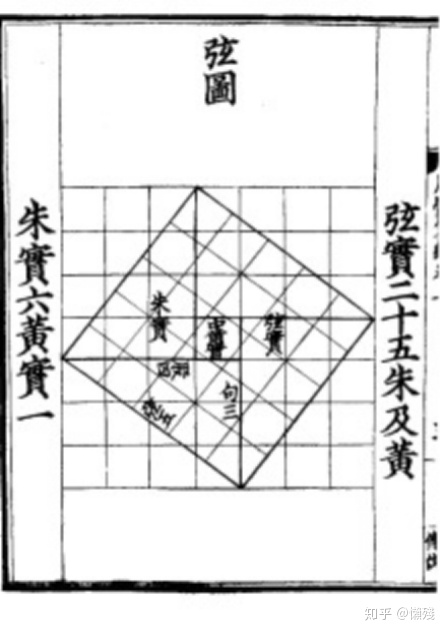
\includegraphics[scale=0.5]{xiantu.jpg}
            \caption{宋赵爽所作弦图。}
            %\lable{xiantu}
        \end{figure}

    \section{勾股定理的现代形式}
        勾股定理的现代现代语言表述如下\cite{Shiye}:
        \begin{thm}[勾股定理]
            直角三角形斜边的平方等于两腰的平方和。

            设直角三角形 ABC,其中 $\angle ACB = \pi / 2$,
            则有:
            \begin{equation}
                AB^2 = BC^2 + AC^2.
            \end{equation}
        \end{thm}

        满足式 (1) 的整数称为\emph{勾股数}。
        一些勾股数如下表:\\[3pt]

        \begin{table}[ht]
            \begin{tabular}{|rrr|}
                \hline
                直角边 $a$ & 直角边 $b$ & 斜边 $c$\\
                \hline
                $3$ & $4$ & $5$ \\
                \hline
                $5$ & $12$ & $13$ \\
                \hline
                $8$ & $15$ & $17$ \\
                \hline
            \end{tabular}
            \qquad
            ($a^2 + b^2 = c^2$)
        \end{table}

    \bibliographystyle{plain}
    \bibliography{math}
    
\end{document}


